\documentclass{article}
\usepackage[utf8]{inputenc}
\usepackage{hyperref}
\setlength{\columnsep}{1cm}
\usepackage[margin=0.5in]{geometry}
\usepackage{amsmath}
\usepackage{caption}
\usepackage{subcaption}

\title{Deep Learning Course - Final Project}
\author{Nitsan BenHanoch (208585927), Nir Koren (316443902), Tsvi Tabach (311292304)}
\date{Submitted as a final project report for the DL course, BIU, 2024}

\usepackage{natbib}
\usepackage{graphicx}

\begin{document}

\maketitle

\section{Introduction}

Deep-Learning in healthcare is a hot topic. As deep neural networks become increasingly involved in patient care, these networks must meet several requirements. Such requirements include high precision rate, transparency in their decision-making, and performing effectively even when valuable data is missing.

\subsection{The Dataset}
Kaggle's chest-xray-pneumonia dataset consists of 5,856 lungs X-Ray images of men and children. Each image is labeled either "healthy", "bacterial-infected" or "viral-infected". The data is split between train/set sets. One important issue to note is the classes are not balanced; each set contains a different ratio of images from the different classes.

\subsection{Our Tasks}
In this project, we demonstrate several different deep-learning techniques we learned during the course.

\textbf{Task 1.a. Binary Classification}: we train a CNN on healthy/sick labeled x-ray images of human lungs;

\textbf{Task 1.b. Multiclass classification}: we further improve the CNN to distinguish between bacterial/viral infection;

\textbf{Task 2. Embedding Space:} we apply KNN and t-SNE on embedding vectors we get from the aforementioned networks;

\textbf{Task 3. Anomaly Detection:} having trained on healthy lungs alone, we use auto-encoders to tell if lungs are sick;

\textbf{Task 4. Explainability}: we decipher the model's decision making, e.g. what's important to each layer and neuron.


\subsection{Related Works}
Previous research, such as \href{https://arxiv.org/pdf/1711.05225.pdf}{CheXNet}, study by Rajpurkar et al. (2017), has shown the advantage of using CNN in medical diagnostics. The model proposed in the paper used CNN to output probability of pneumonia with a heat-map localizing the pneumonia areas from chest X-ray images.

\
\section{Task 1.a: Binary Classification}

\subsection{Solution}
\subsubsection{The Task}
In this task, we treat both bacterial and viral images as
\textit{sick}, and train a model to classify \textit{healthy}/\textit{sick} lungs x-ray.

\subsubsection{General approach}
We use several convolution layers, followed by a few dense layers. It is the field's classic and go-to way to classify images. Furthermore, the limited dataset size (approximately 5K images) posses a serious restriction on the complexity of the network, as overly powerful architectures risk significant over-fitting.

\subsubsection{Design}

Our network's architecture mimics the great: we took inspiration from the architecture of the VGG networks family. We tailored their layer sizes to our needs after thorough experimentation, maximizing accuracy, while battling over-fitting. The final network structure is portrayed in Figure~\ref{fig:model_1}.

\textbf{Platform:} we built the model as a Keras Sequential on a kaggle notebook. It ran for $\sim$30 minutes using a P100 GPU. 

\textbf{Loss:} we used binary-crossentropy, as it's classic in the context of binary classification, and it worked for us. 

\textbf{Optimizer:} we used Adam with initial learning rate of 1e-4, but also installed a callback to further lower it on plateau.

\textbf{The Splits}: The train and the 16-images given val were concatenated and re-split into 80\% train and 20\% validation.

\textbf{Limited dataset size:} as said, we only had a few thousand images to train on.
To combat it, we used many augmentation methods to compensate for the lack of data. We also limited the number of epochs.

\textbf{Class imbalance:} the sets had different distributions of labels.
We removed excess data from the train/val sets until each class appeared 50\%; we found that to be more effective than assigning weights. The test-set, having a 62.5\% class imbalance, was left as is.

\begin{figure}
  \centering
  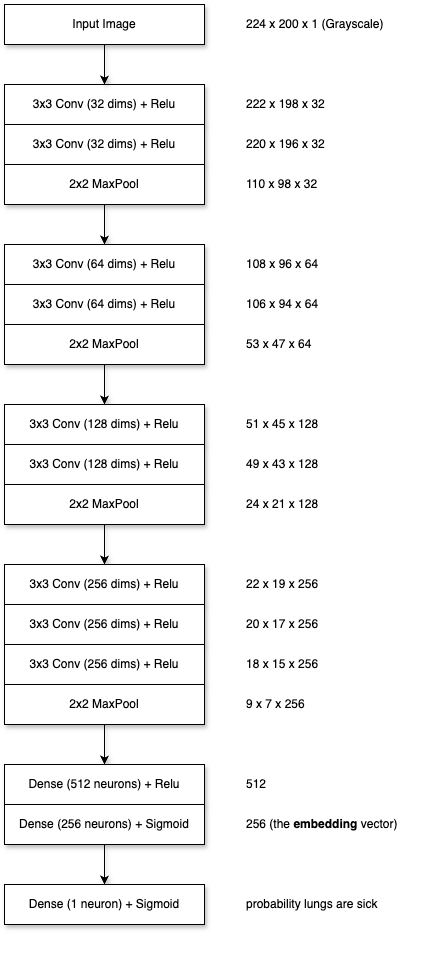
\includegraphics[width=0.45\linewidth, angle=90]{model_1.png}
  \caption{Binary Classification Model}
  \label{fig:model_1}
\end{figure}

\subsection{Experimental results}
Provide information about your experimental settings. What alternatives did you measure? Make sure this part is clear to understand, provide as much details as possible. Provide results with tables and figures.

\subsection{Discussion}
Provide some final words and summarize what you have found from running the experiments you described above. Provide some high level insights.

Note - your project will be evaluated for aspects, including the technique you selected, the rational of the experiments you decided to run, the insights you learned from this process and more. Remember, for the purpose of this course, the process that you demonstrate is very  important.

\subsection{Code}

Please provide a link to your colab notebook.

\
\section{Task 1.2: Multiclass Classification}

\subsection{Solution}
\subsubsection{General approach}
For the multiclass class classification task, We used the ResNet34 architecture with 3 sized classification head. Some alternatives such as Vision Transformer and Dense Net were tested, but the ResNet34 provided the most accuracy on the test set.

\subsubsection{Design}
The ResNet34 architecture we used was taken from the original paper \href{https://arxiv.org/pdf/1512.03385.pdf}{Deep Residual Learning for Image Recognition} by Kaiming He. The architecture includes 34 convolution layers and residual connections between each block. The model is divided into two main components: ResNet34 backbone and 3-sized classification head. A single modification was made to the original ResNet34 architecture: the activation functions were switched from ReLU to GELU to enhance performance.

\textbf{Platform:} We built the model as a Pytorch class on a kaggle notebook. It ran for 20 epochs and took $\sim$9 minutes using a P100 GPU. 

\textbf{Loss:} We used cross-entropy loss, a go-to loss function for classification tasks.

\textbf{Optimizer:} We used AdamW with an initial learning = 1e-3, weight decay = 0.005

\textbf{Scheduler:} We used a Warmup Cosine Schedule with 5 warmup steps

\textbf{The Splits}: For a more representative validation set we moved 400 samples from the training dataset to the validation dataset. At last, we had 4816 training samples, 416 validation samples, and 624 test samples.

\begin{figure}
  \centering
  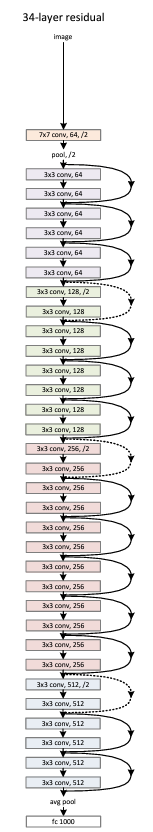
\includegraphics[width=0.15\linewidth, angle=90]{resnet.png}
  \caption{ResNet34 architecture from the original paper}
  \label{fig:resnet}
\end{figure}

\subsection{Experimental results}
The ResNet34 model underwent 20 epochs of training, showcasing a gradual improvement in both training and validation accuracies. Initial epochs demonstrated a significant loss decrease and accuracy improvement, stabilizing as the epochs progressed. The final recorded training accuracy was 81.89\%, with a loss of 0.4253, whereas the validation accuracy peaked at approximately 79.33\% with a similar loss range. The model weights were saved every time the validation accuracy peaked.

The test performance was independently evaluated using the model weights that achieved the best validation accuracy. This assessment resulted in a test accuracy of 83.28\% and a loss of 0.5847, demonstrating robust generalization.

\subsubsection{Comparison to Alternatives}
Several alternative architectures were evaluated, including Vision Transformer, DenseNet, and fine-tuning of pretrained models. Ultimately, the non-pretrained ResNet34 model was selected as it surpassed all other options in performance. Our primary hypothesis for its superior performance is that the residual connections within the ResNet34 help mitigate the vanishing/exploding gradient problem, thus enabling the construction of a deeper network that excels in classification tasks. Additionally, the pretrained models were initially trained on datasets significantly different from ours, such as ImageNet. This discrepancy likely contributed to the poorer performance observed when fine-tuning these models compared to using a freshly initialized network.

We implemented data augmentation techniques as a strategy to prevent overfitting. However, our experimental results did not show an improvement in test accuracy from these augmentations. 

Furthermore, we experimented with using the Stochastic Gradient Descent (SGD), and regular Adam optimizers, but this approach resulted in reduced accuracies compared to our baseline AdamW optimizer.

\subsubsection{Visualizations}
Training and validation loss and accuracy over epochs were plotted, with the final test loss and accuracy ~\ref{fig:resnet_training_trends}.
Additionally, a confusion matrix on the test set was plotted to visually assess the relationships and misclassifications between classes.

\[
\begin{array}{c|cccc}
\text{True/Predicted} & \text{Normal} & \text{Bacteria} & \text{Virus} \\
\hline
\text{Normal} & 189 & 17 & 28 \\
\text{Bacteria} & 9 & 231 & 2 \\
\text{Virus} & 14 & 33 & 101 \\
\end{array}
\]


\begin{figure}
  \centering
  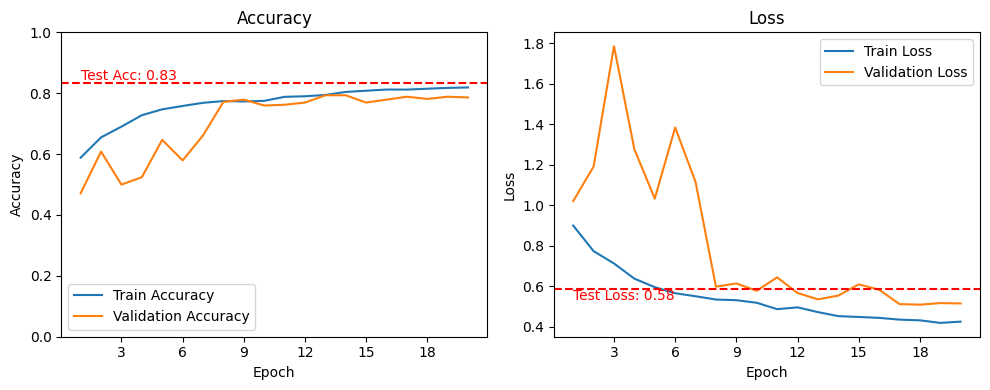
\includegraphics[width=0.8\linewidth, angle=0]{resnet_training_trends.png}
  \caption{ResNet34 training trends}
  \label{fig:resnet_training_trends}
\end{figure}

\subsection{Discussion}
Our exploration validated the non-pretrained ResNet34 as the optimal choice for multiclass classification on the chest-xray-pneumonia dataset. Moreover, selecting the right optimizer and learning rate decay schedule is crucial for optimal performance. Further research into hyperparameter optimization could significantly enhance results.

\subsection{Code}

\href{https://colab.research.google.com/drive/1FQ7bfbL8da7DRQiRvmgwdZXTTDB8sq8w}{Testing Notebook}
\href{https://colab.research.google.com/drive/1Tn58ilSmOiaNIyFNw5BHlqye3YQIMplX#scrollTo=fSeq-k2n1jHI}{Training Notebook}


\
\section{Task 2: Model Embeddings and Visualization}
\subsection{Task 1.b}
\subsubsection{Embedding and KNN classification}
In Task 1.b, we employed a ResNet34 model for multiclass classification purposes. This architecture generates embeddings as 1000-dimensional vectors, which are subsequently inputted into a final linear layer with dimensions 1000x3 for classification. Leveraging these embeddings, we trained a K-Nearest Neighbors (KNN) classifier using the same training dataset as in Task 1.b. We configured the KNN model to utilize 7 neighbors, which achieved an accuracy of 70.03\% on the test set. Additionally, a confusion matrix on the test set was plotted to visually assess the relationships and misclassifications between classes using KNN classifier.


\[
\begin{array}{c|cccc}
\text{True/Predicted} & \text{Normal} & \text{Bacteria} & \text{Virus} \\
\hline
\text{Normal} & 97 & 55 & 82 \\
\text{Bacteria} & 3 & 226 & 13 \\
\text{Virus} & 1 & 33 & 114 \\
\end{array}
\]

\subsubsection{Classes Visualization}
To visualize how the trained network perceives the classes within the dataset, we extracted the embeddings produced by the ResNet34 backbone. These embeddings were then visualized using the t-SNE technique, facilitated by the t-SNE library, to represent the high-dimensional vector space in a two-dimensional plot. As illustrated in Figure \ref{fig:t_sne_1b}, the plot reveals a distinct separation between the Normal and non-Normal classes. Additionally, there is a moderate but discernible linear separation between the Virus and Bacteria classes.

\begin{figure}
  \centering
  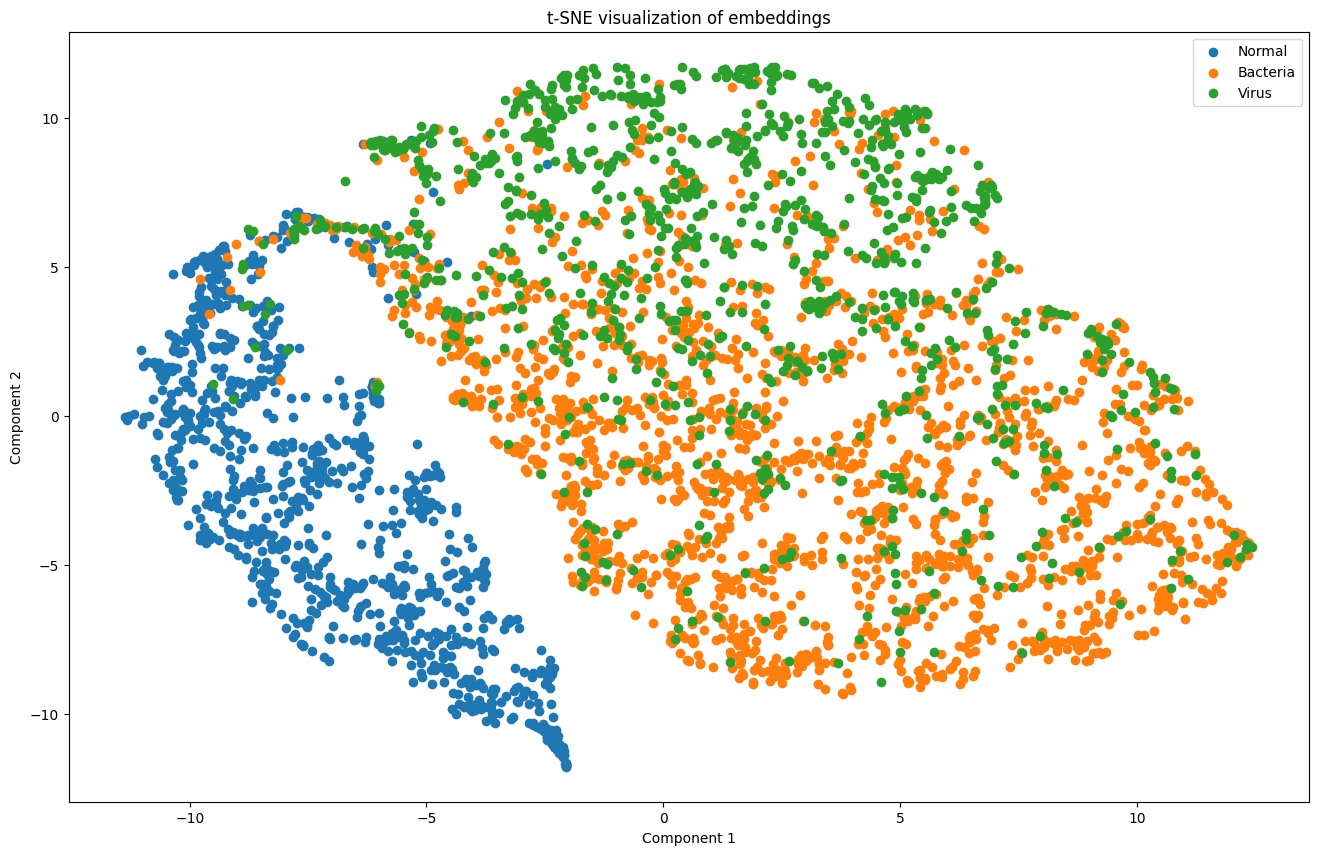
\includegraphics[width=0.55\linewidth, angle=0]{t_sne_1b.png}
  \caption{T-sne visualization of the classes}
  \label{fig:t_sne_1b}
\end{figure}

\subsection{Code}

Please provide a link to your colab notebook.


\
\section{Task 3: Anomaly Detection}

\subsection{Solution}
\subsubsection{General approach}
Describe your preferred approach to solve the problem. what alternatives you plan to try and why. 

\subsubsection{Design}
Provide some general information about your code, platform, how long it took you to train it, technical challenges you had, Loss functions, Optimizers, Architecture, and more.

\subsection{Experimental results}
Provide information about your experimental settings. What alternatives did you measure? Make sure this part is clear to understand, provide as much details as possible. Provide results with tables and figures.

\subsection{Discussion}
Provide some final words and summarize what you have found from running the experiments you described above. Provide some high level insights.

Note - your project will be evaluated for aspects, including the technique you selected, the rational of the experiments you decided to run, the insights you learned from this process and more. Remember, for the purpose of this course, the process that you demonstrate is very  important.

\subsection{Code}

Please provide a link to your colab notebook.


\
\section{Task 4: Explainability in Deep Learning}

\subsection{Solution}
\subsubsection{General approach}
For the explainability of the network in Assignment 1.a, we employed three main approaches: visualizing the receptive fields that correspond to the maximum activations of various filters, generating heatmaps through the occlusion of different classes (Normal and Pneumonia), and synthesizing inputs that trigger high activations in specific layer neurons.

\subsubsection{Receptive Fields Corresponding to Maximum Activations}
In this approach, we selected one of the later convolutional layers (conv2d) of the model. For each of the five filters in this layer, we processed ten images from the dataset. During each forward pass, we identified the point of maximum activation for each filter (a single value from the filter's output) and calculated the corresponding receptive field. We then visualized these receptive fields to gain insights into what the network focuses on during the forward pass. See Figure \ref{fig:receptive_fields} for the plots. We can conclude from the plots that every filter is "looking" for some feature of the image. For example, filter 1 reacts the most for the left lung, while filter 2 reacts the most to the spine.

\subsubsection{Heatmaps by Occlusion}
This method provides insights into the network's decision-making process. We selected two images, one labeled "Normal" and the other "Pneumonia," and applied a masking technique where different areas of the images were obscured with a zero mask of size 90 pixels. This process generated 14,985 masked variations for each image. Each masked image was then processed through the network, and the predicted probabilities were recorded, creating a probability map of size 111x216 for each image. We adjusted the Normal image's probability map by converting the values to 1-value, aligning it with the Pneumonia map, where values closer to 0 indicate critical features (poor model accuracy) and values closer to 1 indicate non-critical features (high model accuracy). As depicted in Figure \ref{fig:occlusion}, the analysis reveals that the network focuses on a large portion of the lungs when classifying a Normal image and concentrates more on the central parts of the lungs for a Pneumonia image, despite high overall precision indicating that the model can utilize multiple areas effectively.

\subsubsection{Synthesizing Inputs}
This approach involves selecting a single image from the dataset and a specific layer within the network. We initiated 64 distinct "training" sessions, using the chosen image as the starting input with its pixels set as trainable parameters. For each session, a different filter from the selected layer was targeted, and gradient ascent was employed to maximize the filter's activation in response to the input. This method helps identify the visual patterns and features that each filter within the layer is most responsive to. As shown in Figure \ref{fig:synth_images}. Each session consisted of 1000 epochs, with a notably high learning rate of 10,000.0. Although this rate may seem unusually large, it was necessary to effect significant modifications to the input image.


\begin{figure}
  \centering
  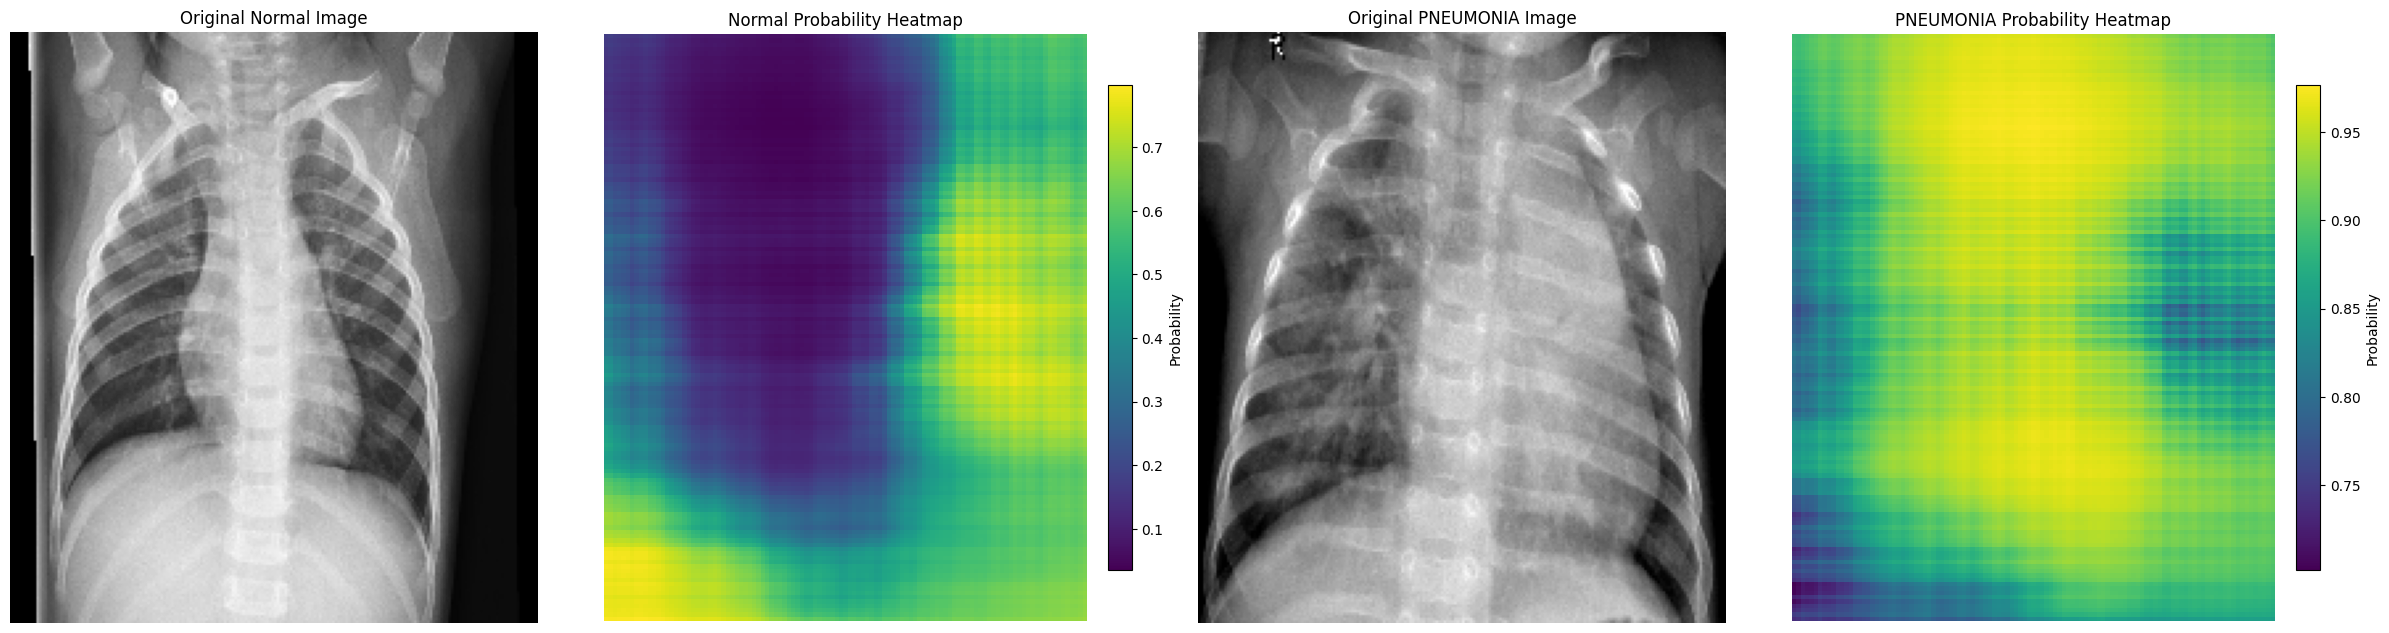
\includegraphics[width=0.95\linewidth, angle=0]{occlusion.png}
  \caption{Heatmaps by Occlusion}
  \label{fig:occlusion}
\end{figure}

\begin{figure}
     \centering
     \begin{subfigure}[b]{0.45\textwidth}
         \centering
         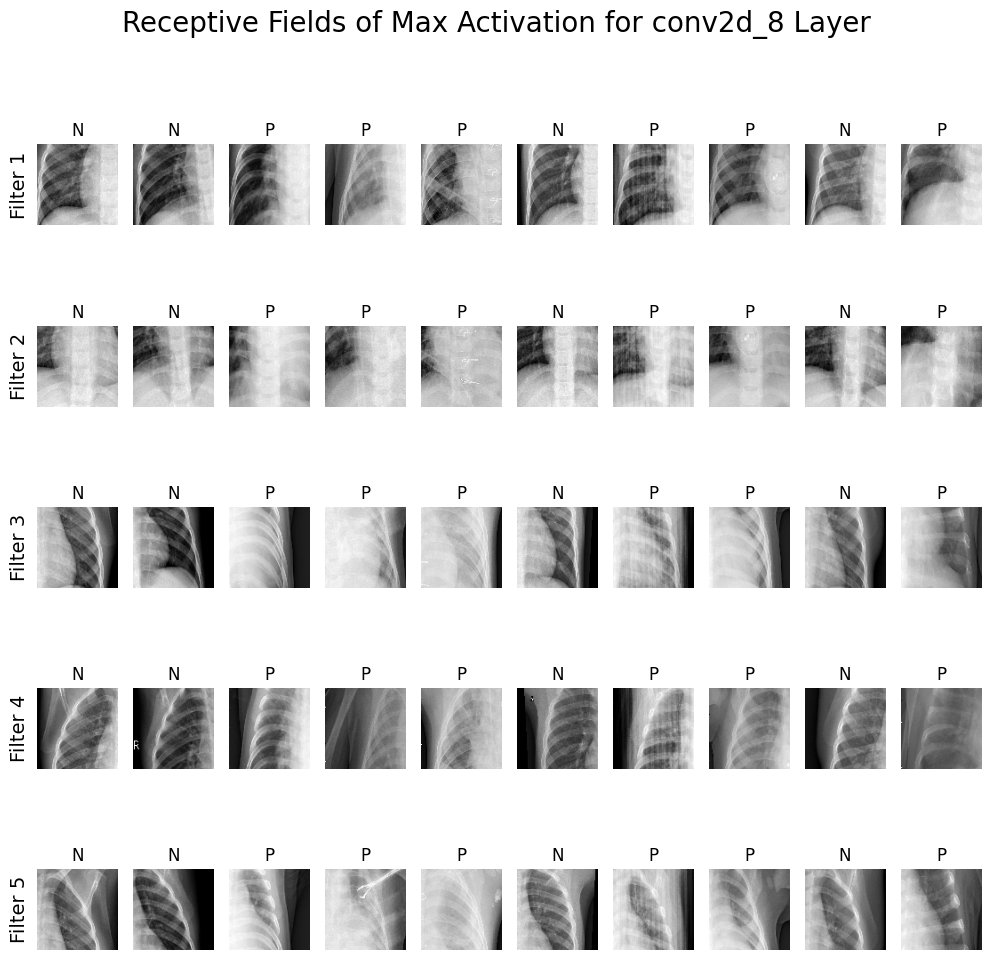
\includegraphics[width=1.0\linewidth, angle=0]{receptive_fields.png}
          \caption{Receptive fields of max activation. (N=Normal, P=Pneumonia)}
          \label{fig:receptive_fields}
     \end{subfigure}
     \hfill
     \begin{subfigure}[b]{0.45\textwidth}
         \centering
         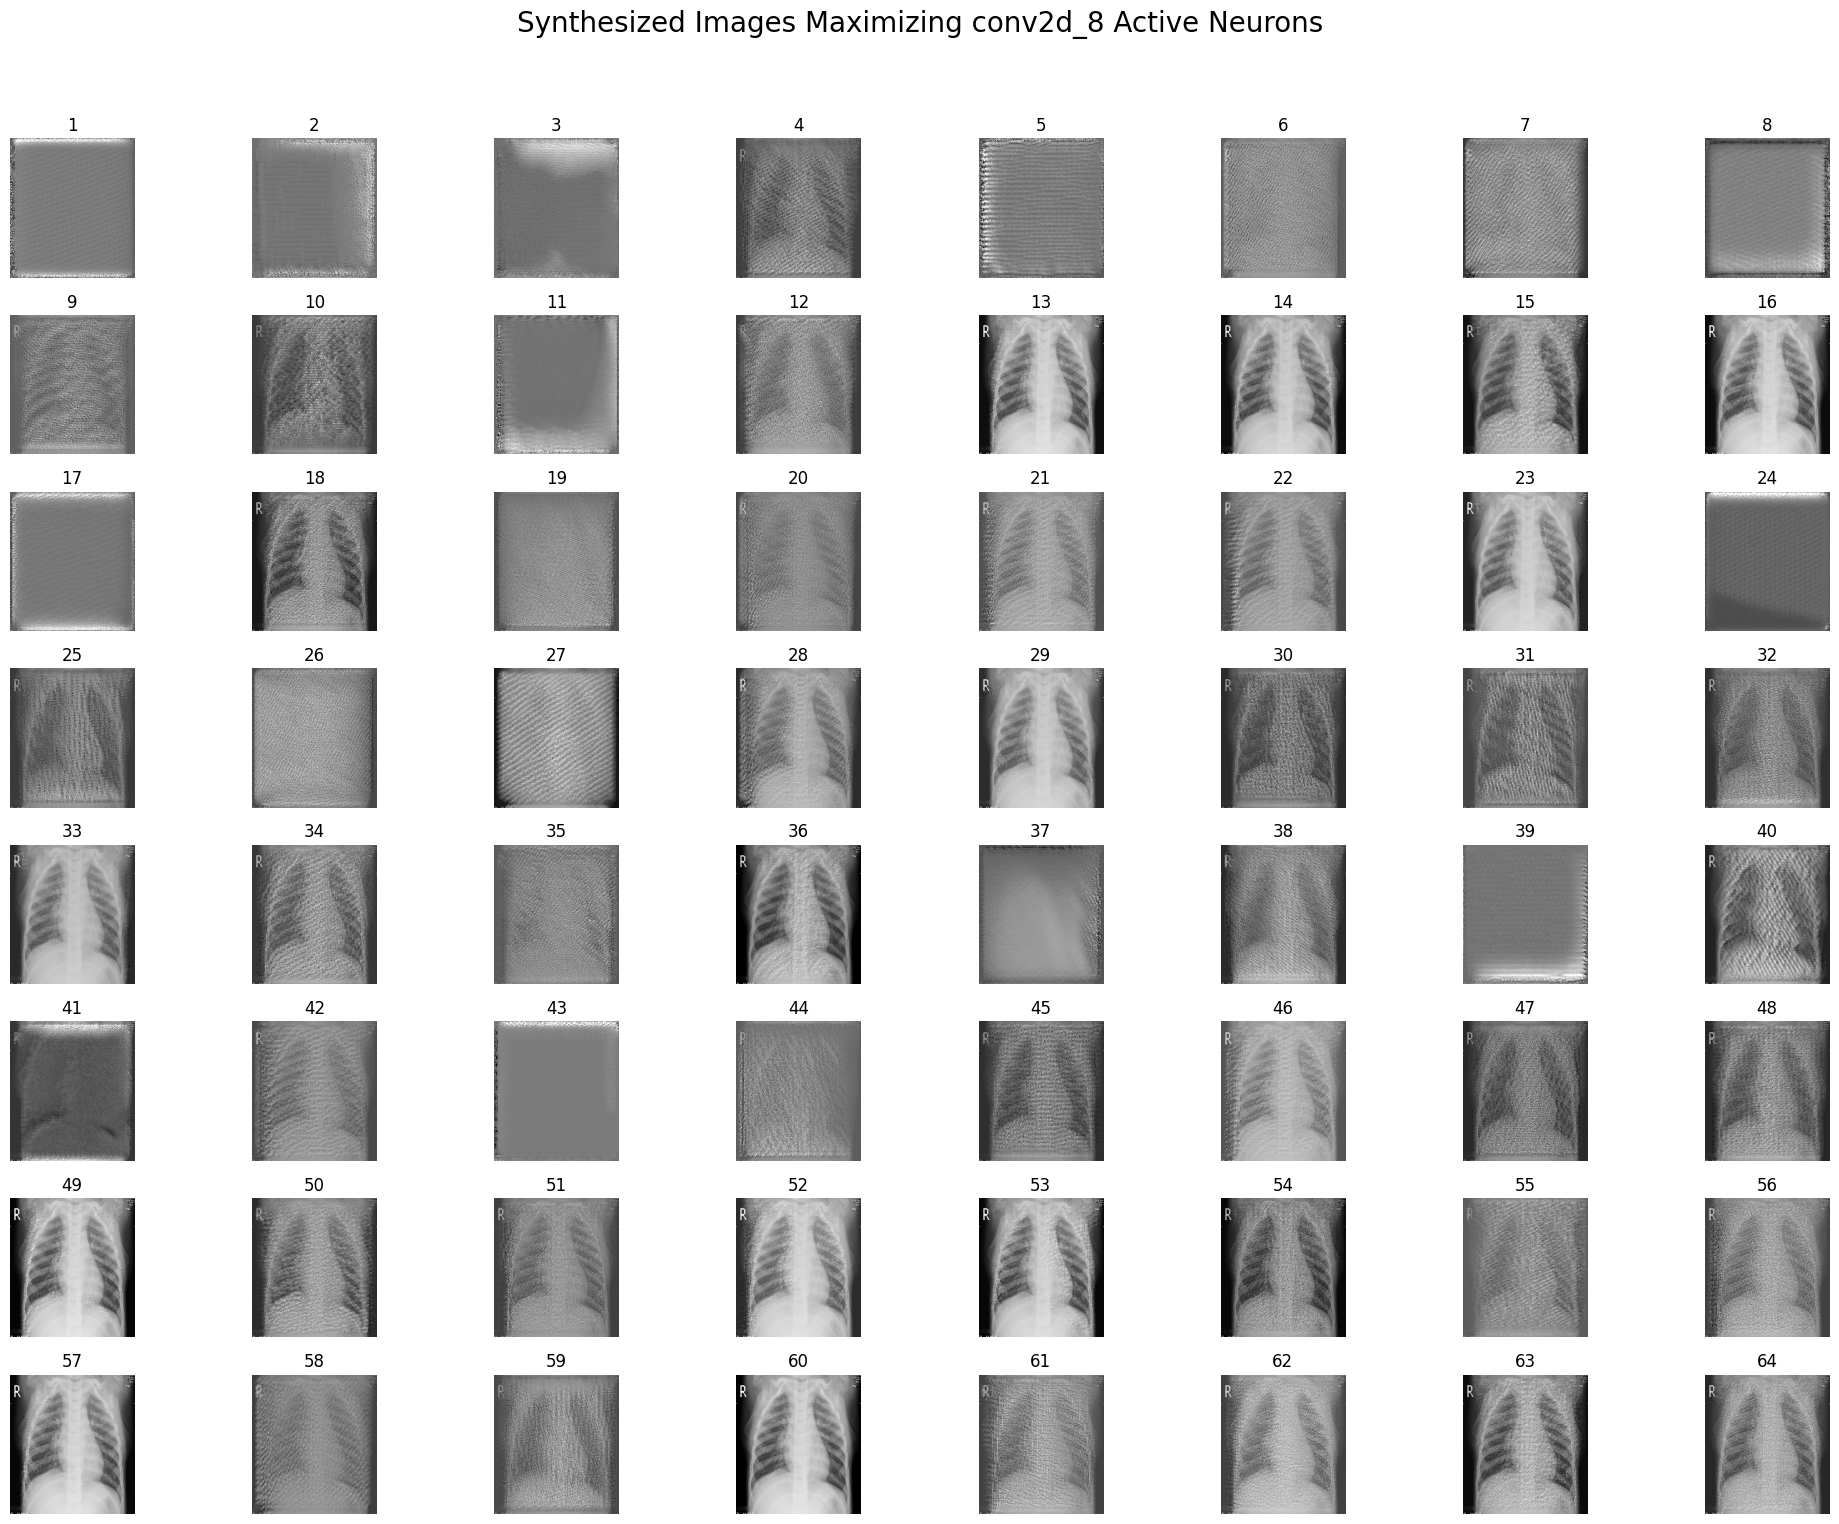
\includegraphics[width=1.1\linewidth, angle=0]{synth_images.png}
          \caption{Synthesizing inputs that cause high activation}
          \label{fig:synth_images}
     \end{subfigure}
     
        \caption{}
        \label{fig:three Explainability approaches}
\end{figure}


\subsection{Code}

Please provide a link to your colab notebook.

Good luck!!
\bibliographystyle{plain}
\bibliography{references}
\end{document}